\section{Implementation costs and larger radii}
\label{sec:implementation}
\subsection{Where the implementation saves time}
The counter-and-heap implementation changes how greedy scores are maintained. Once a vertex becomes covered, its contribution is removed from the affected counters; the algorithm need not recompute complete neighborhood intersections after each selection. Under the same primary, secondary and final tie priorities, the new implementation produces the same complete landmark sequence as the reference. Consequently, the implementation comparison isolates computation and storage costs rather than a change in solution quality.

Figure~\ref{fig:phases} decomposes the $r=1$ Ratio runs into input, neighborhood/data-structure preparation, selection and output. The five SNAP graphs use five repetitions per implementation; uk-2002 uses three. Every phase is summarized by its own median. The whole-process measurement is an external start-to-exit time and additionally includes startup, shutdown and other overhead. Independent phase medians therefore need not sum to the median whole-process time.

\begin{figure}[H]
\centering
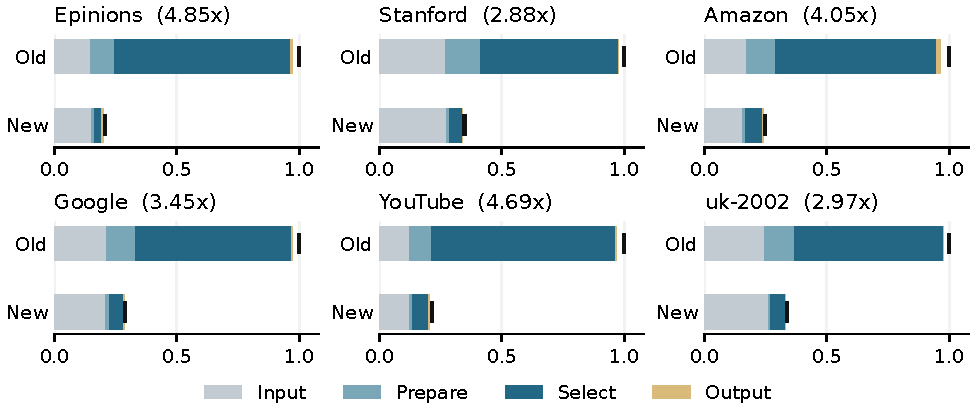
\includegraphics[width=\linewidth]{implementation_phases.pdf}
\caption{Ratio phase costs at $r=1$, divided by the reference implementation's median whole-process time on each graph. Black ticks mark whole-process times; panel labels give whole-process speedups. Stacked segments are independently computed phase medians.}
\label{fig:phases}
\end{figure}

\paragraph{Selection and preparation.}
The selection phase improves by approximately $9.7$--$22.9\times$ on the five SNAP graphs; on uk-2002 it improves by $10.3\times$. Neighborhood/data-structure preparation also decreases. These savings explain why the implementation advantage remains substantial even though the choice of landmarks is unchanged. The report's machine-readable phase table retains all absolute measurements, including input and output, rather than only the normalized figure.

\paragraph{The input floor.}
Input costs change little compared with selection costs. For example, uk-2002 input takes $67.75$ seconds in the reference and $72.12$ seconds in the new implementation, while selection falls from $168.27$ to $16.40$ seconds. Input alone accounts for approximately $77\%$ of the new whole-process time. Thus a larger selection-stage speedup does not imply an equally large end-to-end speedup. The whole-process speedup is $2.97\times$ on this graph, including its input cost.

\paragraph{Measurement controls.}
Both implementations use the same graph, vertex order, greedy strategy and compiler flags on the same pinned core. Coverage, objective value and ordered landmark output are independently checked. This phase comparison uses 50 Ratio records on the five SNAP graphs and six on uk-2002, a subset of the manuscript's four-strategy validation collection.

\clearpage
\subsection{Complete multi-radius rerun cohort}
At larger radii, explicitly represented neighborhoods become much larger. Table~\ref{tab:radius} reports every condition in the completed Stanford reference-implementation rerun cohort: the full graph and five sampled views, each at $r=2,3$. The 50,000-vertex views use seeds 20261105 and 20261107; the 100,000-vertex views use these seeds and 20261106. The table lists each size, seed and radius combination in the cohort.

\begin{table}[H]
\centering\smalltablefont\setlength{\tabcolsep}{4pt}
\caption{All twelve multi-radius conditions. Entries are three-run medians. View seed suffixes 05/06/07 denote 20261105/06/07. Speedup is old/new whole-process time; saved memory is $100(1-\mathrm{new}/\mathrm{old})$.}
\label{tab:radius}
\begin{tabular}{@{}lrrrrrrr@{}}
\toprule
View / seed & $r$ & Old (s) & New (s) & Speedup & Old GiB & New GiB & Saved (\%) \\
\midrule
50k / 05 & 2 & 886.9 & 40.6 & 21.82 & 63.57 & 5.77 & 90.9 \\
50k / 05 & 3 & 1458.6 & 106.2 & 13.74 & 101.75 & 8.31 & 91.8 \\
50k / 07 & 2 & 969.7 & 50.9 & 19.04 & 68.08 & 6.13 & 91.0 \\
50k / 07 & 3 & 1600.0 & 202.1 & 7.92 & 109.82 & 8.99 & 91.8 \\
100k / 05 & 2 & 1567.1 & 41.6 & 37.64 & 74.19 & 6.59 & 91.1 \\
100k / 05 & 3 & 4718.7 & 179.6 & 26.27 & 204.33 & 17.80 & 91.3 \\
100k / 06 & 2 & 1947.0 & 59.2 & 32.87 & 95.95 & 8.53 & 91.1 \\
100k / 06 & 3 & 3386.8 & 159.2 & 21.27 & 171.08 & 14.39 & 91.6 \\
100k / 07 & 2 & 1547.1 & 41.8 & 36.99 & 73.54 & 6.54 & 91.1 \\
100k / 07 & 3 & 4628.0 & 185.6 & 24.94 & 205.78 & 17.88 & 91.3 \\
Full graph & 2 & 2243.2 & 62.5 & 35.87 & 107.24 & 9.43 & 91.2 \\
Full graph & 3 & 6205.4 & 221.3 & 28.04 & 251.46 & 21.66 & 91.4 \\
\bottomrule
\end{tabular}

\end{table}

\paragraph{Observed scaling.}
The new implementation is faster in all twelve conditions, with speedups from $7.92$ to $37.64\times$. Peak RSS decreases by $90.9$--$91.8\%$. The full-graph endpoints highlighted in the manuscript belong to this wider set of paired observations. The table lists individual seeds to capture the neighborhood-density variation between sampled views.

\paragraph{Resource limits and timing.}
The reference implementation runs serially with a 320\,GiB address-space limit and unlimited wall/CPU time. The new implementation uses a 64\,GiB address-space limit. Table~\ref{tab:radius} reports the elapsed time and observed peak RSS of the completed runs.

Whole-process time covers native process startup, input, preprocessing, greedy selection, output and destruction. Independent validation time is excluded for both implementations. The runs use the same pinned server core. The separate pilot is excluded from the 36 formal reference runs.

\paragraph{Output agreement.}
The completion audit verifies all 36 formal reference runs, including independent coverage/cost checks and complete ordered-output agreement with the new implementation. Original source and binary identities are unchanged. These comparisons measure implementation efficiency at larger landmark radii.
